\begin{figure}[htbp]
    \centering

    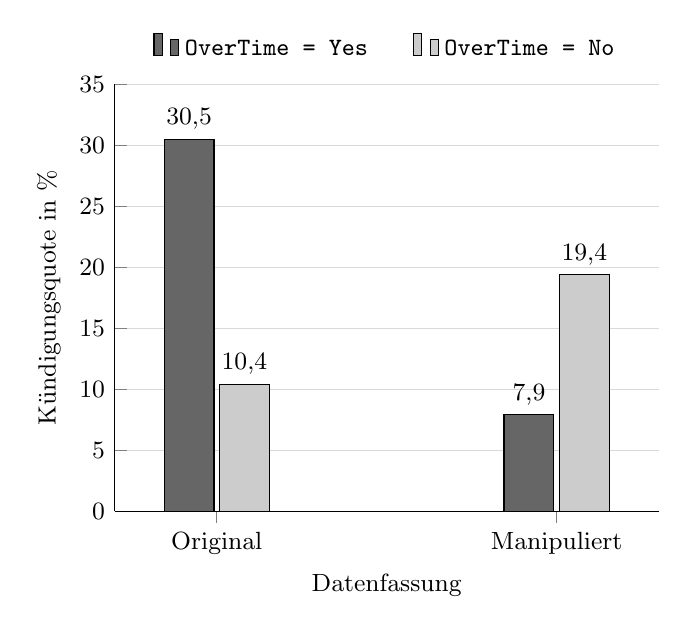
\begin{tikzpicture}
    \begin{axis}[
        width=0.82\textwidth,
        height=7cm,
        ybar,
        bar width=18pt,
        ymin=0,
        ymax=35,
        ytick={0,5,10,15,20,25,30,35},
        ylabel={Kündigungsquote in \%},
        ylabel style={font=\small},
        symbolic x coords={Original,Manipuliert},
        xtick=data,
        xlabel={Datenfassung},
        xlabel style={font=\small},
        tick label style={font=\small},
        enlarge x limits=0.30,
        width=0.7\textwidth,
        ymajorgrids=true,
        grid style={draw=black!15},
        axis lines*=left,
        legend style={
            at={(0.5,1.03)},
            anchor=south,
            legend columns=2,
            draw=none,
            font=\small,
            /tikz/every even column/.append style={column sep=0.5cm}
        },
        nodes near coords,
        nodes near coords style={
            font=\small,
            /pgf/number format/fixed,
            /pgf/number format/precision=1
        },
        every node near coord/.append style={
            /pgf/number format/use comma
        }
    ]

    \addplot[
        draw=black,
        fill=black!60
    ] coordinates {
        (Original,30.5)
        (Manipuliert,7.9)
    };

    \addplot[
        draw=black,
        fill=black!20
    ] coordinates {
        (Original,10.4)
        (Manipuliert,19.4)
    };

    \legend{
        \texttt{OverTime = Yes},
        \texttt{OverTime = No}
    }

    \end{axis}
    \end{tikzpicture}

    \caption[Kündigungsquoten vor und nach der Manipulation]{
        Kündigungsquoten nach \texttt{OverTime} im ursprünglichen und
        manipulierten Datensatz. Die Randverteilungen bleiben in beiden Fassungen identisch, mit 416 Beschäftigten mit und 1054 ohne Überstunden sowie unveränderter Gesamtkündigungsquote; umgekehrt wird allein die Richtung des Zusammenhangs zwischen beiden Variablen.
    }
    \label{fig:overtime-manipulation}
\end{figure}